\documentclass[letterpaper, 6 pt, journal, twoside]{IEEEtran}
\usepackage[english]{babel}
\usepackage[utf8]{inputenc}
\usepackage{amsmath}
\usepackage{graphicx}
\usepackage[colorlinks=true, allcolors=blue]{hyperref}
\usepackage[capitalize]{cleveref}

\begin{document}

\begin{figure}
    \centering
    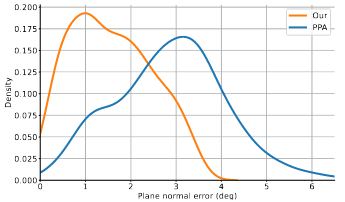
\includegraphics[width=6cm]{images/Figure_3.png} 
    \caption{Plane normal error distributions for our method and PPA.}
    \label{fig:Fig3}
\end{figure}

effect is strongly attenuated, showing evidence that the per-
spective distortion have been effectively compensated. PPA
performs better than Ortho, but the radial pattern is still par-
tially visible.

\subsection{Plane orientation estimation}

    Since in the Orthographic model $\phi$ is the azimuth angle of $\Vec{n}$, the linear constraint 
\begin{equation}
        (\begin{array}{ccc} \sin{\phi} & \cos{\phi} & 0 \end{array}) . \Vec{n} = 0
\end{equation}

is usually considered in photo-polarimetric stereo ap-
proaches or iso-depth contour tracing. If we know that at
least K $>$ 3 pixels observe the same plane, we can use such
constraint to recover the plane normal $\Vec{n}$ (in camera refer-
ence frame) from the (corrected) $\phi_j$ observed at each pixel
by solving:

\begin{equation}
        (\begin{array}{cccc} 
        (\sin{\phi_1} & \cos{\phi_1} & 0 ) & R_1^T \\
        (\sin{\phi_2} & \cos{\phi_2} & 0 ) & R_2^T \\
        & . \\
        & . \\
        & . \\
        (\sin{\phi_K} & \cos{\phi_K} & 0 ) & R_K^T \\
        \end{array})  
        \Vec{n} = \Vec{0}
\end{equation}

as a Linear Least-Squares problem. Note that the system is
under-determined in the Orthographic model because all the
rays are parallel ($R_1 , . . . R_k$ are identities) and all the pixels
would observe the same $\phi$. In the PPA model, instead, a
similar costraint is provided (See Eq. 7 in \cite{chen2022perspective}).
    
    In \cref{fig:Fig3} we plotted the the estimated plane normal er-
ror distribution against the Ground Truth data in the PPA
dataset. The Ortho model is not present in the plot for the
reasons discussed before. Also in this case, our mean abso-
lute error is lower (1.57\textdegree vs. 2.89\textdegree) and with less variabil-
ity. This reflects a better estimation of the AoLP due to the
correction applied by the tilted polarizer model.

\subsection{Normal estimation}

    Our work is not a SfP method, so evaluating its valid-
ity based on how well a normal field is reconstructed has to
be done with care. We recall that the azimuth angle of $\Vec{n}$ is
equal to the AoLP $\phi$ up to a (unavoidable) $\pi$-ambiguity, and
an additional $\pi/2$-ambiguity depending if specular or diffuse
reflection dominates. Since in the plane dataset the specu-
lar reflection is dominant, we used the following function
to relate the DoLP $\rho$ with zenith angle $\theta$ and the index of
refraction $\mathbf{n}$ :

\begin{equation}
        \rho(\mathbf{n},\theta) = a \frac{2\sin^2\theta\cos\theta\sqrt{\mathbf{n}^2 - \sin^2\theta}}{\mathbf{n}^2-\sin^2\theta-\mathbf{n}^2\sin^2\theta+2\sin^4\theta}
        \label{eq:Eq16}
\end{equation}

where a is a scale parameter we added to the original formu-
lation shown in \cite{atkinson2006recovery} to account for a possible diffuse compo-
nent of reflection and other nonlinear contribution like the
Umov’s effect [\cite{kupinski2019angle}, \cite{umow1905chromatische}].
To show the validity of our approach, the idea is to test
how well our model allows the recovery of surface normals
in ideal conditions, i.e. with an oracle that removes the
ambiguities and provides a close estimate of the unknown
parameters $\mathbf{n}$, a in \cref{eq:Eq16}) Since we know the Ground
Truth normals of both the datasets, we manually estimated
the best value of the two parameters and computed the er-
rors considering the minimum error among all the possi-
ble ambiguities. We compare the resulting normal field
against: (i) the \textit{orthographic} model using the same ora-
cle as our method (i.e. estimated function $\rho$ and optimal
disambiguator); (ii) \textit{Smith} et al. [26]; (iii) \textit{Smith corrected}
with our pre/post processing to account for projective cam-
era, and (iv) SfPW [19], a Deep CNN with a multi-head
self-attention module and viewing encoding “to account for
non-orthographic projection in scene-level”. We used the
original author implementation pre-trained on their SPW
Dataset.

    We listed the MAE and RMSE of the estimated normals
in \cref{tab:Tab2}. Normals recovered with our projective model are
significantly more accurate than the others. This is not sur-
prising, since we assume to have an oracle that resolves all
the unknowns we usually face when doing SfP. The impor-
tant thing to notice here is the improvement against the or-
thographic model that uses the same oracle. In other words,
properly accounting for non orthographic projection is cru-
cial to reduce the error, no matter how sophisticated is the
method applied to solve the ambiguities. Moreover, the
\textit{Smith corrected} performs better than the original one be-
cause can now accounts for non-orthographic cameras. We
stress that this correction was performed as pre/post pro-
cessing without modifying any other part of the method. Fi-
nally, SfPW performs well but not better than the “simple”
Orthographic model. Considering that SfPW can take into
account non-orthographic cameras, we expected a lower er-
ror in this experiment. In general, SfP is difficult to solve
without posing additional strong priors to the reconstructed
scene, and learning-based method can only try to resolve
the ambiguities based on what observed on the training set,
with the risk of overfitting specific 3D structures. In \cref{fig:Fig4}
we show a qualitative example of the obtained normal field.

\begin{figure}
    \centering
    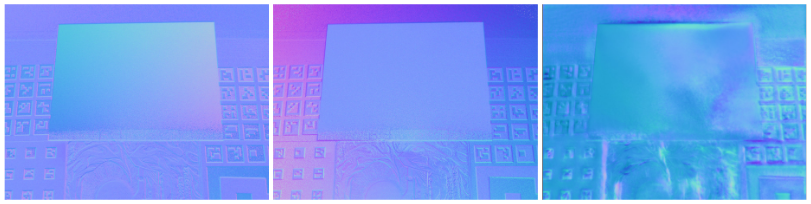
\includegraphics[width=18cm]{images/Figure_4.png} 
    \caption{Qualitative comparison of the estimated normal field with methods Ortho (left), Our (center), and SfPW (right) on an instance of the PPA dataset. Errors are computed only inside the plane area but we kept the rest of the scene for visualization purposes. Note how a radial pattern is visible in the Ortho model since the distortion due to the ray orientation is not accounted for. SfPw performs poorly because it has been trained on a much noisier dataset and apparently is not able to generalize to simpler scenarios.}
    \label{fig:Fig4}
\end{figure}


\subsection{Other datasets}

    We also tested our method on a dataset of general ob-
jects presented in [3]. In this case it is difficult to provide an
oracle because it contains scenes with different kind (dif-
fuse/specular) and degrees of polarization. So, we limit
our test to the observation of how the pre/post processing
can improve an existing SfP method. Similarly to what we
did with planes dataset, we compare \textit{Smith}, \textit{Smith corrected},
\textit{SfPW} and \textit{DeepSfP} [3]. The latter method is a Deep model
assuming an orthographic camera, so potentially is a valid
candidate to be corrected with our model. However, at the
time of writing, the code and pre-trained weights were not
publicly available so we report here the results shown in
the original paper. \cref{tab:Tab3} show the MAE of the estimated
normals in the whole dataset. SfPW is the best performing
method, followed by DeepSfP. It is interesting to observe
that, also in this case, Smith corrected with our model ob-
tains a significant improvement.
{\small
\bibliographystyle{IEEEtran}
\bibliography{Ref}
}

\end{document}
